\chapter{\projName (think of a name for the system)} \label{chap:system}

In this chapter I would present the majority of the work we have done.
From a design perspective, implementation, and evaluation.

\section{Building Blocks}

For each one, present:
\begin{itemize}
    \item A bit of the theory behind it
    \item A basic proof of concept (maybe even bash scripts)
    \item Integration with \texttt{runc} and our system (yet to be named)
    \item A micro-benchmark of this feature.
\end{itemize}

This first section introduces the key building blocks of that make up \projName.
For each one of them we cover the theoretical concepts, the problem they try to solve, their implementation (and integration with \criu and \runc if existent), together with a targeted benchmark.

\cs{Describe the evaluation setting, versions etc.}

\subsection{Diskless Migration}

\subsection{Iterative Migration}

% Brief Introduction
As introduced in \S

Implemented in \criu we find a series of features that enable us to perform iterative migrations of running processes.
This is, periodically snapshot the state of the process without altering it until some condition is triggered, that in turn checkpoints the container and restores it elsewhere.
The key idea being that all the heavy work for the snapshot (\textit{i.e.} capturing the memory state and transferring it) will have already been done in previous iterations, hence minimizing the application downtime.

In the previous paragraph we have assumed that transfers across consequent snapshots will be smaller in size, otherwise the $n$-th dump would not be any faster than the first one, and we would be wasting a lot of bandwidth since the same information would be sent repeatedly.
This reduction in size can be achieved through memory tracking, a procedure through which memory pages written between dumps are marked as \emph{dirty} and hence included in the following transfer.
Therefore, to implement efficient iterative migration we need:
\begin{enumerate}
    \item \textbf{Pre-Dump:} A procedure to snapshot the memory of the process without stopping it (note that, at this point, we don't need all the other details).
    \item \textbf{Memory Tracking:} A procedure to keep track of the memory changes in a process' address space.
    \item \textbf{Parent Directory:} A procedure to link together subsequent dumps so that they can be correctly re-interpreted at restore time.
\end{enumerate}

The first step during an iterative migration consists on dumping \emph{all} of the process memory to an image file.
This allows for a baseline from which smaller \emph{incremental} dumps are performed.
Note that, at this point, we are not interested in capturing the whole state, hence the usage of the \texttt{pre-dump} command in CRIU.

Memory tracking in CRIU~\cite{criu-memory-tracking} is done by means of a kernel functionality introduced in 2013~\cite{criu-memory-tracking-lwn}.
It consists of two steps: first we ask the kernel to keep track of memory changes on a per-process basis by writing a $4$ to \texttt{/proc/\$pid/clear\_refs} and, after a while, reading the \texttt{/proc/\$pid/pagemap} file and checking the \textit{soft-dirty} bit for each page table entry (PTE).
Internally, in the first step the kernel clears all soft-dirty bits \emph{and} the writable ones per each PTE for the given process id (PID).
Subsequent writes to any page will trigger a page fault, a call to \texttt{pte\_mkdirty}, and therefore the \textit{soft-dirty} bit will be set.
During the second step, at memory dump time, if this bit has not been set, the memory page needs not to be transferred again.
To enable this functionality in \criu, we must use the \texttt{--track-mem} flag.

One last key step required to achieve efficiency and correctness upon restore is to link the actual dump (or pre-dump) with the one preceding it, it's \emph{parent}.
For a pre-dump, \texttt{--prev-images-dir} indicates \criu to look for exsiting dumps in the specified path, and perform the bit-checking described in the previous paragraphs.
Upon restore, links among successive dumps are pieced together to successfully restore the freshest version of the running program.

In order to perform a micro-benchmark of this functionality we consider two different scenarios: a simple counter written in \texttt{C} (see Listing~\ref{code:c-counter}), and a \redis in-memory database.
For each scenario we perform two pre-dumps, and a final dump, and report the size of the \texttt{pages-1.img} file (which contains the memory dump).
We test a static setting in which we don't change the memory during successive dumps which acts as a baseline, and a dynamic one in which, between each dump, we modify the contents of the process memory.
For the counter, the static setting starts the program and goes to sleep, whereas the dynamic one indeed updates the counter every other second.
For the database, we initially pre-load it with $1e7$ key-value pairs (around 300 MB of data) and then either do nothing, or run a \texttt{redis-benchmark} which alters around $1\%$ of the key pairs.

\begin{figure}[h!]
    \centering
    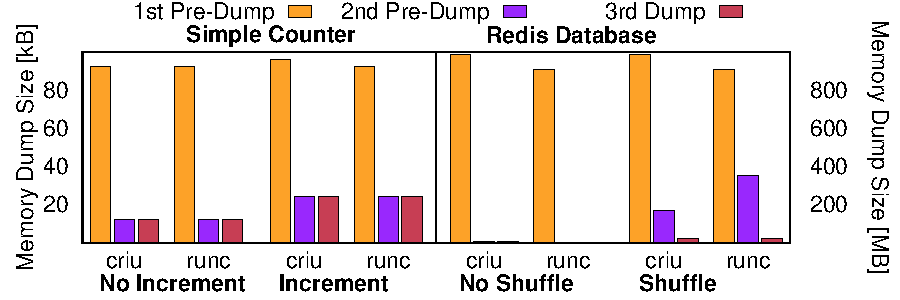
\includegraphics[width=.8\textwidth]{figs/iterative-migration-microbenchmark/iterative_migration_microbenchmark.pdf}
    \caption[Size of the memory image for iterative dumps.]{Size of the dumped memory image when performing iterative dumps. For the counter experiment we report the results in kB (left axis) and for the redis one we report the results in MB (right axis). We compare the results when using \runc or purely \criu.\label{fig:iterative-migration-microbenchmark}}.
\end{figure}

We present our results in Figure~\ref{fig:iterative-migration-microbenchmark}.


\subsubsection*{Aside: Memory Deduplication}

Maybe not an aside, but putting it here to remember

\subsection{Remote Migration}

\subsection{Checkpointing TCP Connections}

\subsubsection*{Aside: Checkpointing Established TCP Connections}

\section{Checkpointing Multiple Containers}

To be done.
A necessary first step is to manage the namespaces and IPs as we do now.

\section{Putting it All Together}

A bit of a walkthrough of the final implementation
